\documentclass[11pt]{article}
\usepackage[margin=0.8in]{geometry}
\usepackage{amsmath, amssymb}
\usepackage{enumitem}
\usepackage{booktabs}
\usepackage{xcolor}
\usepackage{multicol}
\usepackage{float}
\usepackage{tikz}
\usetikzlibrary{arrows.meta, positioning, calc}

\definecolor{garnet}{HTML}{73000A}
\definecolor{black90}{HTML}{363636}
\definecolor{atlantic}{HTML}{466A9F}
\definecolor{congaree}{HTML}{1F414D}
\definecolor{horseshoe}{HTML}{65780B}
\definecolor{rose}{HTML}{CC2E40}

\color{black90}

\newcommand{\important}[1]{\textcolor{garnet}{\textbf{#1}}}
\newcommand{\concept}[1]{\textcolor{atlantic}{\textbf{#1}}}
\newcommand{\formula}[1]{\begin{center}\fcolorbox{garnet}{white}{\parbox{0.9\linewidth}{#1}}\end{center}}
\newcommand{\intuition}[1]{\begin{center}\fcolorbox{atlantic}{blue!3}{\parbox{0.9\linewidth}{\textcolor{atlantic}{\textbf{Intuition:}} #1}}\end{center}}
\newcommand{\example}[1]{\begin{center}\fcolorbox{horseshoe}{green!3}{\parbox{0.9\linewidth}{\textcolor{horseshoe}{\textbf{Example:}} #1}}\end{center}}

\setlength{\parskip}{4pt}
\setlength{\parindent}{0pt}

\title{\color{garnet}\textbf{Quiz 2 Study Guide --- Lectures 4--7}\\[4pt]
\large CSCE 775 --- Spring 2026}
\author{J.C.\ Vaught}
\date{}

\begin{document}
\maketitle
\thispagestyle{empty}

\textbf{Quiz format:} 1 math problem (50\%) + conceptual questions (50\%).
Strategy: nail the conceptual questions, get partial credit on the math.

\vspace{1em}

% ======================================================================
\part{Lecture 4: Model-Free RL}
\textit{Covers Sutton \& Barto Ch.\ 5.1--5.7, 6.1--6.5, 7.1--7.3}
% ======================================================================

\section{Big Picture}

\concept{Model-free RL} means learning from \textit{experience} without knowing the transition function $p(s',r \mid s,a)$. Two tasks:

\begin{itemize}[nosep]
    \item \textbf{Prediction (policy evaluation):} estimate $v_\pi$ or $q_\pi$ for a given $\pi$
    \item \textbf{Control:} find the optimal policy $\pi_*$
\end{itemize}

Three families of methods, each with a different \textit{target} for the update:

\begin{table}[H]
\centering
\begin{tabular}{llll}
\toprule
\textbf{Method} & \textbf{Target} & \textbf{Bias} & \textbf{Variance} \\
\midrule
Monte Carlo & $G_t$ (full return) & None & High \\
TD(0) & $R_{t+1} + \gamma V(S_{t+1})$ & Yes (bootstrap) & Low \\
$n$-step TD & $R_{t+1} + \cdots + \gamma^{n-1}R_{t+n} + \gamma^n V(S_{t+n})$ & Medium & Medium \\
\bottomrule
\end{tabular}
\end{table}

% --------------------------------------------------
\section{Monte Carlo Methods (Ch.\ 5)}
% --------------------------------------------------

\subsection{MC Prediction}

Estimate $v_\pi(s) = \mathbb{E}_\pi[G_t \mid S_t = s]$ by averaging \textit{sampled returns}.

\formula{
\textbf{MC Incremental Update:}\quad
$V(S_t) \leftarrow V(S_t) + \alpha\bigl(G_t - V(S_t)\bigr)$
}

\begin{itemize}[nosep]
    \item \textbf{First-visit MC:} average $G_t$ only the \textit{first} time $s$ appears in an episode.
    \item \textbf{Every-visit MC:} average $G_t$ every time $s$ appears.
    \item Must wait until the episode ends to compute $G_t$. Does \textit{not} work for continuing (non-episodic) tasks.
\end{itemize}

\intuition{MC is like grading a restaurant after eating the entire meal. You wait until the end, then assign a score to the whole experience. Accurate (unbiased), but your one meal might have been unusually good or bad (high variance).}

\example{A robot plays 3 episodes starting from state $A$. It gets total returns $G = -5, -3, -7$. After first-visit MC: $V(A) = (-5 + -3 + -7)/3 = -5$. Incrementally: start $V(A)=0$, after ep.\ 1: $V(A) = 0 + 1(-5-0) = -5$. After ep.\ 2: $V(A) = -5 + \frac{1}{2}(-3-(-5)) = -4$. After ep.\ 3: $V(A) = -4 + \frac{1}{3}(-7-(-4)) = -5$.}

\subsection{MC Control (On-Policy)}

Use $Q(s,a)$ instead of $V(s)$ because we cannot derive a policy from $V$ without a model.

\formula{
\textbf{Policy from Q:}\quad $\pi(s) = \arg\max_a Q(s,a)$
}

\important{$\varepsilon$-greedy exploration:}
\[
\pi(a \mid s) =
\begin{cases}
1 - \varepsilon + \varepsilon/|\mathcal{A}(s)| & \text{if } a = \arg\max_{a'} Q(s,a') \\
\varepsilon/|\mathcal{A}(s)| & \text{otherwise}
\end{cases}
\]

The on-policy MC control algorithm: generate episode $\to$ compute returns backward $\to$ update $Q(S_t,A_t)$ $\to$ improve policy to $\varepsilon$-greedy w.r.t.\ new $Q$.

\intuition{$\varepsilon$-greedy is like a food critic who \textit{usually} goes to their favorite restaurant (exploit, prob $1-\varepsilon$) but \textit{sometimes} tries a random place (explore, prob $\varepsilon$). Without exploration, you might never discover the best option.}

\example{With $\varepsilon = 0.1$ and 4 actions, the greedy action gets probability $0.9 + 0.1/4 = 0.925$. Each non-greedy action gets $0.1/4 = 0.025$. Sum: $0.925 + 3(0.025) = 1$.}

\subsection{On-Policy vs Off-Policy}

\begin{itemize}[nosep]
    \item \textbf{Behavior policy $b$:} the policy used to collect data.
    \item \textbf{Target policy $\pi$:} the policy we want to evaluate/improve.
    \item \textbf{On-policy:} $b = \pi$.
    \item \textbf{Off-policy:} $b \neq \pi$. Can reuse data from other policies. Requires importance sampling.
\end{itemize}

% --------------------------------------------------
\section{Temporal-Difference Learning (Ch.\ 6)}
% --------------------------------------------------

\subsection{TD(0) Prediction}

\important{Key idea:} update toward a \textit{bootstrapped} target instead of waiting for $G_t$.

\formula{
\textbf{TD(0) Update:}\quad
$V(S_t) \leftarrow V(S_t) + \alpha\bigl[\underbrace{R_{t+1} + \gamma V(S_{t+1})}_{\text{TD target}} - V(S_t)\bigr]$
}

The quantity $\delta_t = R_{t+1} + \gamma V(S_{t+1}) - V(S_t)$ is the \textbf{TD error}.

\intuition{TD is like updating your restaurant rating after \textit{each course}, not waiting for the full meal. After the appetizer, you adjust your expectation based on what you just experienced + your guess about the rest. Faster feedback, but your guess about dessert might be wrong (biased).}

\example{States $A \to B$ with $r=0$, $\gamma=1$, $\alpha=0.1$. Initially $V(A)=0$, $V(B)=0.75$.

TD update: $V(A) \leftarrow 0 + 0.1[0 + 1(0.75) - 0] = 0.075$.

TD immediately propagates $B$'s value back to $A$ after one step. MC would need to wait for the episode to finish.}

\important{MC vs TD:}
\begin{itemize}[nosep]
    \item MC: unbiased, high variance, needs full episodes.
    \item TD: biased (initially), low variance, learns online step-by-step.
    \item TD bootstraps from its own estimate $\Rightarrow$ can propagate value information faster.
\end{itemize}

\subsection{SARSA --- On-Policy TD Control}

\formula{
\textbf{SARSA Update:}\quad
$Q(S_t,A_t) \leftarrow Q(S_t,A_t) + \alpha\bigl[R_{t+1} + \gamma Q(S_{t+1},A_{t+1}) - Q(S_t,A_t)\bigr]$
}

Name comes from the quintuple $(S_t, A_t, R_{t+1}, S_{t+1}, A_{t+1})$.

Both behavior and target policy are $\varepsilon$-greedy. Choose $A_{t+1}$ from $S_{t+1}$ using $\varepsilon$-greedy \textit{before} the update.

\intuition{SARSA asks: ``given what I \textit{actually did} next (including random exploration), how good was my action?'' It's cautious---if exploration might lead off a cliff, SARSA learns to stay away.}

\subsection{Q-Learning --- Off-Policy TD Control}

\formula{
\textbf{Q-Learning Update:}\quad
$Q(S_t,A_t) \leftarrow Q(S_t,A_t) + \alpha\bigl[R_{t+1} + \gamma \max_{a} Q(S_{t+1},a) - Q(S_t,A_t)\bigr]$
}

\important{Key difference:} uses $\max_a Q(S_{t+1},a)$ (greedy) instead of $Q(S_{t+1},A_{t+1})$ ($\varepsilon$-greedy).

\begin{itemize}[nosep]
    \item Behavior policy: $\varepsilon$-greedy (explores).
    \item Target policy: greedy (deterministic).
    \item Off-policy because behavior $\neq$ target.
\end{itemize}

\intuition{Q-learning asks: ``what's the best I \textit{could} do next, assuming I play perfectly from now on?'' It's optimistic---it finds the optimal path even if exploration is risky.}

\important{Cliff Walking Example:}

\begin{center}
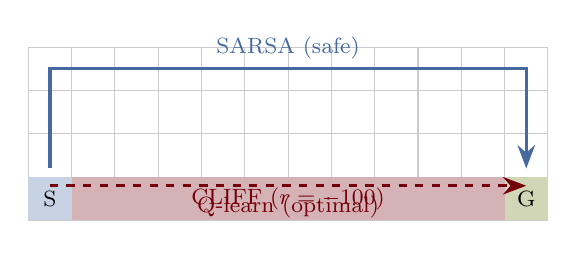
\begin{tikzpicture}[scale=0.55, every node/.style={font=\footnotesize}]
    % Grid
    \foreach \x in {0,...,11} \foreach \y in {0,...,3}
        \draw[black!20] (\x,\y) rectangle (\x+1,\y+1);
    % Cliff
    \foreach \x in {1,...,10}
        \fill[garnet!30] (\x,0) rectangle (\x+1,1);
    \node[garnet] at (6, 0.5) {CLIFF ($r = -100$)};
    % Start/Goal
    \fill[atlantic!30] (0,0) rectangle (1,1);
    \node at (0.5,0.5) {S};
    \fill[horseshoe!30] (11,0) rectangle (12,1);
    \node at (11.5,0.5) {G};
    % Paths
    \draw[-{Stealth}, atlantic, very thick] (0.5,1.2) -- (0.5,3.5) -- (11.5,3.5) -- (11.5,1.2);
    \node[atlantic, above] at (6,3.5) {SARSA (safe)};
    \draw[-{Stealth}, garnet, very thick, dashed] (0.5,0.8) -- (1,0.8) -- (11,0.8) -- (11.5,0.8);
    \node[garnet, below] at (6,0.8) {\footnotesize Q-learn (optimal)};
\end{tikzpicture}
\end{center}

\begin{itemize}[nosep]
    \item SARSA learns a \textit{safer} path (avoids cliff) because it accounts for its own $\varepsilon$-greedy exploration.
    \item Q-learning learns the \textit{optimal} path (close to cliff) because the target policy is greedy.
\end{itemize}

% --------------------------------------------------
\section{$n$-Step Methods (Ch.\ 7)}
% --------------------------------------------------

\formula{
\textbf{$n$-step return:}\quad
$G_{t:t+n} = R_{t+1} + \gamma R_{t+2} + \cdots + \gamma^{n-1}R_{t+n} + \gamma^n V(S_{t+n})$
}

\begin{itemize}[nosep]
    \item $n=1$: TD(0).
    \item $n=\infty$: Monte Carlo.
    \item Typical sweet spot: $n \approx 5$.
\end{itemize}

\textbf{TD($\lambda$)} averages over \textit{all} $n$-step returns with exponentially decaying weights $(1-\lambda)\lambda^{n-1}$. When $\lambda = 0$ you get TD(0); when $\lambda = 1$ you get MC.

\intuition{$n$-step methods are like reading $n$ chapters of a mystery novel before guessing the ending. $n=1$ (TD): guess after the first chapter---fast but unreliable. $n=\infty$ (MC): read the whole book---accurate but slow. Best results come from reading a few chapters ($n\approx 5$) then making an informed guess.}

\example{In a 4-step episode with rewards $r_1=1, r_2=0, r_3=1, r_4=2$ (terminal) and $\gamma=1$:

\textbf{1-step return:} $G_{1:2} = 1 + V(S_2)$\quad (uses one real reward + estimate)

\textbf{2-step return:} $G_{1:3} = 1 + 0 + V(S_3)$\quad (two real rewards + estimate)

\textbf{4-step (MC):} $G_1 = 1+0+1+2 = 4$\quad (all real rewards, no estimate)}

% --------------------------------------------------
\section{Unified View: DP vs TD}
% --------------------------------------------------

\begin{table}[H]
\centering
\begin{tabular}{lll}
\toprule
& \textbf{Full Backup (DP)} & \textbf{Sample Backup (TD)} \\
\midrule
Bellman Expectation for $v_\pi$ & Policy Evaluation & TD Learning \\
Bellman Expectation for $q_\pi$ & Q-Policy Iteration & SARSA \\
Bellman Optimality for $q_*$ & Q-Value Iteration & Q-Learning \\
\bottomrule
\end{tabular}
\end{table}

\important{Key difference:} DP uses the full model (all transitions); TD samples one transition.

% ======================================================================
\newpage
\part{Lecture 5: Deep Learning Fundamentals}
% ======================================================================

\section{Linear Models}

\subsection{Linear Regression}

\formula{
$f(\mathbf{x}, \mathbf{w}, b) = \mathbf{w}^\top \mathbf{x} + b$\qquad
\textbf{Loss:}\quad $\mathcal{L}(\boldsymbol{\theta}) = \frac{1}{2n}\sum_{i=1}^n (y_i - f(\mathbf{x}_i, \boldsymbol{\theta}))^2$
}

\textbf{Analytical solution:} $\mathbf{w}^* = (\mathbf{X}^\top\mathbf{X})^{-1}\mathbf{X}^\top\mathbf{y}$

\textbf{Gradient descent update:} $\mathbf{w} \leftarrow \mathbf{w} - \alpha \nabla_{\boldsymbol{\theta}}\mathcal{L}(\boldsymbol{\theta})$

\intuition{Linear regression fits a line (or hyperplane) that minimizes the total squared distance to the data points. Gradient descent nudges the line toward data points it currently misses most.}

\example{Predicting house price from square footage: $f(x) = w \cdot x + b$. If $w=200, b=50000$, a 1500 sq ft house costs $\$350{,}000$. The loss measures how far off our predictions are from actual prices.}

\subsection{Logistic Regression (Binary Classification)}

\formula{
\textbf{Sigmoid:}\quad $\sigma(z) = \frac{1}{1 + e^{-z}}$\qquad
\textbf{Derivative:}\quad $\sigma'(z) = \sigma(z)(1-\sigma(z))$
}

$P(y=1 \mid \mathbf{x}) = \sigma(\mathbf{w}^\top \mathbf{x})$. Decision boundary where $\mathbf{w}^\top \mathbf{x} = 0$.

\textbf{Loss:} negative log-likelihood (cross-entropy):
\[
\mathcal{L} = -\sum_i \bigl[y_i \log \sigma(\mathbf{w}^\top \mathbf{x}_i) + (1-y_i)\log(1-\sigma(\mathbf{w}^\top \mathbf{x}_i))\bigr]
\]

\intuition{Sigmoid squashes any real number into $(0,1)$---like a dimmer switch that smoothly goes from ``off'' to ``on.'' For $z \gg 0$, output $\approx 1$; for $z \ll 0$, output $\approx 0$. The cross-entropy loss punishes confident wrong answers exponentially.}

\example{Email spam classification: $\mathbf{w}^\top\mathbf{x} = 3.5 \Rightarrow \sigma(3.5) = 0.97 \Rightarrow$ 97\% chance of spam. If actually spam ($y=1$): loss $= -\log(0.97) = 0.03$ (small). If not spam ($y=0$): loss $= -\log(0.03) = 3.5$ (large penalty for being confidently wrong).}

\subsection{Softmax (Multi-class)}

\[
P(y = i \mid \mathbf{x}) = \frac{e^{\mathbf{w}_i^\top \mathbf{x}}}{\sum_{j=1}^C e^{\mathbf{w}_j^\top \mathbf{x}}}
\]

% --------------------------------------------------
\section{Neural Networks}
% --------------------------------------------------

\subsection{Architecture}

A 2-layer network: $f(\mathbf{x}) = \mathbf{W}^{(2)}\sigma(\mathbf{W}^{(1)}\mathbf{x})$

\important{Activation functions must be non-linear}, otherwise the network collapses to a linear model regardless of depth.

\intuition{A neural network without non-linear activations is just matrix multiplication stacked: $\mathbf{W}_2(\mathbf{W}_1 \mathbf{x}) = (\mathbf{W}_2\mathbf{W}_1)\mathbf{x} = \mathbf{W}'\mathbf{x}$. No matter how many layers, it is still linear. Non-linear activations let the network ``bend'' the decision boundary into curves, spirals, and arbitrary shapes.}

\example{XOR problem: inputs $(0,0)\to 0$, $(0,1)\to 1$, $(1,0)\to 1$, $(1,1)\to 0$. No single line separates the classes. A 2-layer network with ReLU can solve this; a linear model cannot.}

\subsection{Common Activation Functions}

\begin{table}[H]
\centering
\begin{tabular}{lll}
\toprule
\textbf{Name} & \textbf{Formula} & \textbf{Notes} \\
\midrule
Sigmoid & $\sigma(x) = 1/(1+e^{-x})$ & Output in $(0,1)$; vanishing gradient \\
Tanh & $\tanh(x)$ & Output in $(-1,1)$ \\
ReLU & $\max(0,x)$ & Most common; dead neurons possible \\
Leaky ReLU & $\max(0.1x, x)$ & Fixes dead neuron problem \\
\bottomrule
\end{tabular}
\end{table}

\subsection{Universal Function Approximation}

With enough hidden units, a neural network can approximate \textit{any} continuous function to arbitrary precision. Does \textit{not} guarantee convergence of training.

\subsection{Backpropagation}

Chain rule applied layer by layer. For output layer weights:
\[
\frac{\partial E}{\partial W_{ij}^{(2)}} = -(y_i - \hat{y}_i)\,h_j
\]
For hidden layer weights, errors propagate backward through the chain rule.

\intuition{Backpropagation is the chain rule applied systematically. Think of a pipeline: raw material $\to$ factory 1 $\to$ factory 2 $\to$ product. If the product is bad, you trace blame backward: How much did factory 2 mess up? Given factory 2's error, how much did factory 1 contribute? Each factory adjusts proportionally to its blame.}

\subsection{Hyperparameters vs Parameters}

\begin{itemize}[nosep]
    \item \textbf{Parameters:} learned from data (weights, biases).
    \item \textbf{Hyperparameters:} set before training (learning rate, \# layers, \# neurons, $\varepsilon$, etc.).
\end{itemize}

% --------------------------------------------------
\section{Overfitting and Regularization}
% --------------------------------------------------

\begin{table}[H]
\centering
\begin{tabular}{ll}
\toprule
\textbf{Technique} & \textbf{How it works} \\
\midrule
Train/Val/Test split & Monitor val loss; never train on test \\
Weight regularization & Add $\lambda \sum W_{ij}^2$ to loss \\
Dropout & Randomly zero out neurons during training \\
Data augmentation & Rotations, flips, noise to increase data \\
Early stopping & Stop when validation error starts rising \\
\bottomrule
\end{tabular}
\end{table}

\intuition{Overfitting is like memorizing the textbook word-for-word instead of understanding the concepts. You ace the homework (training set) but fail the exam (test set). Regularization techniques force the model to learn \textit{general patterns} instead of memorizing noise.}

\example{A polynomial of degree 100 can pass through 100 training points perfectly (training loss $= 0$) but wildly oscillates between them. A degree-2 polynomial has higher training loss but generalizes much better to new data.}

% --------------------------------------------------
\section{Optimization}
% --------------------------------------------------

Loss surface is non-convex: local minima, saddle points.

\begin{table}[H]
\centering
\begin{tabular}{ll}
\toprule
\textbf{Optimizer} & \textbf{Update Rule} \\
\midrule
SGD & $\mathbf{w} \leftarrow \mathbf{w} - \alpha \nabla E$ \\
SGD + Momentum & $\mathbf{v} \leftarrow \mu\mathbf{v} + \alpha\nabla E$;\quad $\mathbf{w} \leftarrow \mathbf{w} - \mathbf{v}$ \\
ADAM & Adaptive lr per parameter using mean \& variance of gradients \\
\bottomrule
\end{tabular}
\end{table}

\textbf{Stochastic GD:} compute gradients on random mini-batches instead of full dataset.

\subsection{Residual Networks (ResNets)}

Skip connections: $\text{output} = F(\mathbf{x}) + \mathbf{x}$. Smooths the loss surface; enables training very deep networks (100+ layers).

\subsection{Batch Normalization}

Normalize activations to mean 0, std 1 within each mini-batch. Stabilizes training, allows larger learning rates.

\intuition{
\textbf{SGD with momentum} is like a ball rolling downhill---it accumulates speed and can roll past small bumps (local minima). \textbf{ADAM} is like a ball that also adjusts its speed independently in each direction, moving faster along flat dimensions and slower along steep ones.

\textbf{ResNets:} In deep networks, gradients can vanish layer by layer. Skip connections provide a ``highway'' for gradients to flow directly backward, so even layer 100 gets a strong learning signal.

\textbf{Batch norm:} Without it, each layer's input distribution shifts as earlier layers update (internal covariate shift). Batch norm re-centers activations each step, so layers don't have to chase a moving target.
}

\example{Training a 20-layer network: without skip connections, the gradient at layer 1 is $\approx 0$ (vanishing gradient). With skip connections, the gradient flows through the shortcut: $\frac{\partial}{\partial \mathbf{x}}[F(\mathbf{x}) + \mathbf{x}] = F'(\mathbf{x}) + \mathbf{I}$. The identity $\mathbf{I}$ ensures the gradient is at least 1.}

% ======================================================================
\newpage
\part{Lecture 6: PyTorch}
% ======================================================================

\section{Key Concepts (Likely Conceptual Questions)}

\begin{enumerate}[nosep]
    \item \textbf{Automatic differentiation:} define forward pass; PyTorch computes backward pass (gradients) automatically via computation graph.
    \item \textbf{Tensor:} multi-dimensional array (like numpy ndarray), but tracks gradients.
    \item \textbf{Computation graph:} directed graph of operations. Forward pass builds it; \texttt{loss.backward()} traverses it backward.
    \item \textbf{\texttt{.detach()}:} removes a tensor from the computation graph (stops gradient flow).
    \item \textbf{Data type:} PyTorch expects \texttt{float32}. Convert before or after creating tensors.
    \item \textbf{\texttt{loss.item()}:} extract scalar value without keeping the computation graph (prevents memory leak).
    \item \textbf{\texttt{nnet.train()} vs \texttt{nnet.eval()}:} training mode enables dropout and batch norm updates; eval mode disables them.
    \item \textbf{Saving/loading:} \texttt{torch.save(nnet.state\_dict(), path)} saves only parameters, not architecture.
\end{enumerate}

\section{Training Loop Pattern}

\begin{enumerate}[nosep]
    \item \texttt{optimizer.zero\_grad()} --- clear old gradients
    \item Forward pass: \texttt{output = nnet(input)}
    \item Compute loss: \texttt{loss = criterion(output, target)}
    \item Backward pass: \texttt{loss.backward()}
    \item Update weights: \texttt{optimizer.step()}
\end{enumerate}

\section{ResNet in PyTorch}

Residual block: two linear layers + skip connection. Requires input dim = hidden dim (or use a linear projection). Forward: $\mathbf{x} \leftarrow \text{ReLU}(F(\mathbf{x}) + \mathbf{x})$.

\section{Gradient Checking}

Finite differences: $\frac{\partial f}{\partial \theta_i} \approx \frac{f(\theta_i + h) - f(\theta_i)}{h}$ for small $h$ (e.g., $10^{-5}$). Verify each layer independently, then compose.

\intuition{PyTorch's autograd is like having an accountant who watches every arithmetic operation you do (forward pass) and records it in a ledger (computation graph). When you call \texttt{.backward()}, the accountant traces the ledger in reverse to compute exactly how much each input contributed to the final result. \texttt{.detach()} tells the accountant to stop recording---useful for targets that should be treated as constants (like in DQN).}

\example{The 5-step PyTorch training loop maps to calculus:

1.~\texttt{zero\_grad()} $\to$ erase old $\nabla_\theta$\quad
2.~Forward $\to$ compute $\hat{y}$\quad
3.~Loss $\to$ compute $\mathcal{L}$\quad
4.~\texttt{backward()} $\to$ compute $\nabla_\theta \mathcal{L}$\quad
5.~\texttt{step()} $\to$ $\theta \leftarrow \theta - \alpha\nabla_\theta\mathcal{L}$

Forgetting \texttt{zero\_grad()} accumulates gradients across batches (gradients from batch 2 are added to batch 1's gradients).}

% ======================================================================
\newpage
\part{Lecture 7: DAVI and Deep Q-Networks}
% ======================================================================

\section{Deep Approximate Value Iteration (DAVI)}

When the state space is too large for a table, approximate $v_*(s)$ with a neural network $v_\theta(s)$.

\formula{
\textbf{DAVI Target:}\quad
$y = \begin{cases} \max_a\bigl(r(s,a) + \gamma \sum_{s'} p(s'|s,a)\, v_\theta(s')\bigr) & \text{if } s \text{ non-terminal} \\ 0 & \text{if } s \text{ terminal}\end{cases}$
}

\formula{
\textbf{Loss:}\quad $L(\theta) = \frac{1}{2}(y - v_\theta(s))^2$\qquad
\textbf{Gradient:}\quad $\nabla_\theta L = (y - v_\theta(s))\nabla_\theta v_\theta(s)$
}

\important{Do NOT differentiate $y$ with respect to $\theta$} even though $y$ depends on $\theta$. Treat $y$ as a fixed target.

\intuition{DAVI is value iteration (from DP) but with a neural network instead of a table. Normally, value iteration updates every state at once using the model. DAVI does the same thing but trains a neural network to approximate the value function. The target $y$ is the ``what the value \textit{should} be'' (one-step lookahead), and we train the network to match it.}

\example{Grid world with 1 million states---too many for a table. DAVI: sample a batch of states, compute targets $y = \max_a[r + \gamma \sum_{s'} p(s'|s,a) v_{\theta^-}(s')]$ using the frozen target network, then do one gradient step to make $v_\theta(s)$ closer to $y$. Repeat.}

\subsection{Target Network}

Problem: target $y$ changes every iteration (non-stationary).

Solution: maintain a separate \textbf{target network} $v_{\theta^-}$ whose parameters are periodically copied from $\theta$. Use $\theta^-$ to compute $y$, train $\theta$.

\intuition{Without a target network, you're chasing a moving target: every time you update $\theta$, the target $y$ changes too (because $y$ depends on $v_\theta$). It's like trying to hit a bullseye that moves every time you throw. The target network freezes the bullseye for $C$ steps, letting you make progress.}

% --------------------------------------------------
\section{Deep Q-Networks (DQN)}
% --------------------------------------------------

Approximate $q_*(s,a)$ with a neural network. Input: state $s$. Output: $Q$-values for all actions (one forward pass).

\formula{
\textbf{DQN Target:}\quad
$y = \begin{cases} r + \gamma \max_{a'} q_{\theta^-}(s', a') & \text{non-terminal} \\ r & \text{terminal}\end{cases}$
}

\formula{
\textbf{DQN Loss:}\quad $L(\theta) = \frac{1}{2}(y - q_\theta(s,a))^2$
}

\subsection{Three Key DQN Innovations}

\begin{enumerate}[nosep]
    \item \important{Target network} ($\theta^-$ updated periodically) --- stabilizes training by making targets less non-stationary.
    \item \important{Experience replay buffer} --- store $(s, a, r, s')$ tuples; sample random mini-batches to decorrelate training data and prevent catastrophic forgetting.
    \item \important{Huber loss} --- clips gradients for large TD errors, preventing instability from large rewards.
\end{enumerate}

\subsection{DQN Ablation (know this!)}

Both replay buffer AND target network are essential. Removing either one drastically hurts performance. DQN also vastly outperforms linear function approximators.

\intuition{DQN = Q-learning + neural network + two tricks.

\textbf{Experience replay:} Instead of learning from experiences in order (which are correlated---consecutive frames in a game look alike), store them in a buffer and sample random mini-batches. This breaks correlations, just like shuffling a deck of flashcards helps you learn better than going in order.

\textbf{Target network + replay} are \textit{both} essential. The ablation study shows removing either one causes catastrophic failure. They solve different problems: replay breaks correlation, target network prevents oscillation.}

\example{Atari Breakout: state = raw pixels (84$\times$84$\times$4 frames). Action = left/right/fire. DQN outputs $Q(s,a)$ for all 3 actions in one forward pass. The replay buffer stores millions of $(s,a,r,s')$ transitions. Every 10{,}000 steps, copy $\theta \to \theta^-$.}

% --------------------------------------------------
\section{DQN Improvements}
% --------------------------------------------------

\begin{table}[H]
\centering
\begin{tabular}{lp{10cm}}
\toprule
\textbf{Method} & \textbf{Key Idea} \\
\midrule
\textbf{Double Q-Learning} &
Two Q-networks: one selects the action, the other evaluates it. Fixes \textit{maximization bias}.
$y = r + \gamma q_{\theta_2}(s', \arg\max_{a'} q_{\theta_1}(s', a'))$ \\
\addlinespace
\textbf{Dueling DQN} &
Split network into value stream $v_\theta(s)$ and advantage stream $A_\theta(s,a)$.
$q(s,a) = v_\theta(s) + A_\theta(s,a)$. Advantage: $A_\pi(s,a) = q_\pi(s,a) - v_\pi(s)$. \\
\addlinespace
\textbf{Prioritized Replay} &
Sample transitions with large TD error more frequently. \\
\addlinespace
\textbf{Rainbow} &
Combines DQN + Double + Dueling + Prioritized + others. Best overall. \\
\addlinespace
\textbf{Agent57} &
First to beat humans on all 57 Atari games. Uses intrinsic curiosity + adaptive discount. \\
\bottomrule
\end{tabular}
\end{table}

\intuition{\textbf{Double Q-learning} fixes maximization bias: if you ask the same person to both nominate and evaluate candidates, they'll be overconfident. Use one network to \textit{pick} the best action, a different network to \textit{score} it.

\textbf{Dueling DQN} separates ``how good is this state?'' ($v(s)$) from ``how much better is this action than average?'' ($A(s,a)$). Many states have similar values regardless of action---the dueling architecture learns this shared value efficiently.}

% ======================================================================
\newpage
\part{Likely Derivation Problems}
% ======================================================================

The math problem is 50\% and is a pure symbolic derivation (no numbers). Here are the most likely candidates with full step-by-step derivations.

% --------------------------------------------------
\section{Derivation 1: MC Incremental Update from Running Average}
% --------------------------------------------------

\textit{``Show that the running-average MC update can be written in incremental form.''}

Start from the sample-mean definition after $n$ visits to state $s$:
\[
V_n = \frac{1}{n}\sum_{k=1}^{n} G_k
\]

Split off the $n$-th return:
\begin{align}
V_n &= \frac{1}{n}\Bigl(G_n + \sum_{k=1}^{n-1} G_k\Bigr)
= \frac{1}{n}\Bigl(G_n + (n-1)\,V_{n-1}\Bigr) \\[4pt]
&= \frac{1}{n}\,G_n + \frac{n-1}{n}\,V_{n-1}
= \frac{1}{n}\,G_n + V_{n-1} - \frac{1}{n}\,V_{n-1} \\[4pt]
&= V_{n-1} + \frac{1}{n}\bigl(G_n - V_{n-1}\bigr)
\end{align}

\formula{
$V_n = V_{n-1} + \alpha_n\bigl(G_n - V_{n-1}\bigr)$ \quad where $\alpha_n = 1/n$

Generalizing to a constant step size: $V(S_t) \leftarrow V(S_t) + \alpha\bigl(G_t - V(S_t)\bigr)$
}

\intuition{This derivation shows that ``take the average of all returns so far'' is equivalent to ``nudge the old estimate toward the new return.'' The key algebraic trick is splitting off the last term from the sum and rewriting $\frac{n-1}{n} = 1 - \frac{1}{n}$.}

% --------------------------------------------------
\section{Derivation 2: $\varepsilon$-Greedy Policy Improvement}
% --------------------------------------------------

\textit{``Prove that for any $\varepsilon$-greedy policy $\pi$, the $\varepsilon$-greedy policy $\pi'$ w.r.t.\ $q_\pi$ is an improvement: $v_{\pi'}(s) \geq v_\pi(s)$.''}

Start with the expected value under $\pi'$:
\begin{align}
q_\pi(s, \pi'(s)) &= \sum_a \pi'(a \mid s)\,q_\pi(s,a)
= \frac{\varepsilon}{|\mathcal{A}|}\sum_a q_\pi(s,a) + (1-\varepsilon)\max_a q_\pi(s,a)
\end{align}

Since $\max_a q_\pi(s,a) \geq \sum_a w_a\, q_\pi(s,a)$ for any convex weights $w_a$ summing to 1, substitute $w_a = \frac{\pi(a \mid s) - \varepsilon/|\mathcal{A}|}{1-\varepsilon}$:
\begin{align}
&\geq \frac{\varepsilon}{|\mathcal{A}|}\sum_a q_\pi(s,a) + (1-\varepsilon)\sum_a \frac{\pi(a \mid s) - \varepsilon/|\mathcal{A}|}{1-\varepsilon}\,q_\pi(s,a) \\[4pt]
&= \frac{\varepsilon}{|\mathcal{A}|}\sum_a q_\pi(s,a) + \sum_a \bigl(\pi(a \mid s) - \varepsilon/|\mathcal{A}|\bigr)\,q_\pi(s,a) \\[4pt]
&= \sum_a \pi(a \mid s)\,q_\pi(s,a) = v_\pi(s)
\end{align}

\formula{
$q_\pi(s,\pi'(s)) \geq v_\pi(s)$ for all $s$. By the \textbf{policy improvement theorem}, this implies $v_{\pi'}(s) \geq v_\pi(s)$ for all $s$.\qquad $\square$
}

\intuition{The trick is showing the $\varepsilon$-greedy action value is at least as good as the old policy. The $\max$ in $\varepsilon$-greedy is $\geq$ any weighted average (including the old policy's weights), because max $\geq$ average.}

% --------------------------------------------------
\section{Derivation 3: Sigmoid Derivative}
% --------------------------------------------------

\textit{``Derive $\frac{d}{dz}\sigma(z)$ where $\sigma(z) = \frac{1}{1+e^{-z}}$.''}

\begin{align}
\sigma(z) &= (1 + e^{-z})^{-1} \\[4pt]
\frac{d\sigma}{dz} &= -(1+e^{-z})^{-2} \cdot (-e^{-z})
= \frac{e^{-z}}{(1+e^{-z})^2} \\[4pt]
&= \frac{1}{1+e^{-z}} \cdot \frac{e^{-z}}{1+e^{-z}}
= \sigma(z) \cdot \frac{(1+e^{-z})-1}{1+e^{-z}} \\[4pt]
&= \sigma(z)\bigl(1 - \sigma(z)\bigr)
\end{align}

\formula{
$\dfrac{d\sigma}{dz} = \sigma(z)\bigl(1-\sigma(z)\bigr)$
}

\intuition{The sigmoid derivative is maximized at $z=0$ (where $\sigma = 0.5$, so $\sigma' = 0.25$) and vanishes for $|z| \gg 0$. This is why deep sigmoid networks suffer from vanishing gradients: each layer multiplies by at most 0.25.}

% --------------------------------------------------
\section{Derivation 4: Gradient of Logistic Regression Loss}
% --------------------------------------------------

\textit{``Derive the gradient of the cross-entropy loss for logistic regression.''}

The log-likelihood for one sample:
\[
\ell = y\log\sigma(\mathbf{w}^\top\mathbf{x}) + (1-y)\log(1-\sigma(\mathbf{w}^\top\mathbf{x}))
\]

Using $\sigma' = \sigma(1-\sigma)$ and abbreviating $\hat{y} = \sigma(\mathbf{w}^\top\mathbf{x})$:
\begin{align}
\frac{\partial \ell}{\partial \mathbf{w}}
&= y \cdot \frac{\hat{y}(1-\hat{y})}{\hat{y}}\,\mathbf{x} + (1-y)\cdot\frac{-\hat{y}(1-\hat{y})}{1-\hat{y}}\,\mathbf{x} \\[4pt]
&= y(1-\hat{y})\,\mathbf{x} - (1-y)\hat{y}\,\mathbf{x}
= (y - \hat{y})\,\mathbf{x}
\end{align}

The loss is \textit{negative} log-likelihood, so the gradient of the loss over $N$ samples:

\formula{
$\nabla_{\mathbf{w}} \mathcal{L} = -\dfrac{1}{N}\displaystyle\sum_{i=1}^N (y_i - \hat{y}_i)\,\mathbf{x}_i
= \dfrac{1}{N}\sum_{i=1}^N (\hat{y}_i - y_i)\,\mathbf{x}_i$
\quad where $\hat{y}_i = \sigma(\mathbf{w}^\top\mathbf{x}_i)$
}

\intuition{The gradient has a beautiful form: $(\hat{y} - y)\mathbf{x}$. The update is proportional to the error ($\hat{y}-y$) in the direction of the input ($\mathbf{x}$). Large errors $\to$ large updates. The key step is using $\sigma' = \sigma(1-\sigma)$ to cancel the denominators from the log derivatives.}

% --------------------------------------------------
\section{Derivation 5: Backpropagation for a 2-Layer Network}
% --------------------------------------------------

\textit{``Derive the weight gradients for a 2-layer network.''}

Network: $\hat{\mathbf{y}} = \mathbf{W}^{(2)}\,\mathbf{h}$ where $\mathbf{h} = \sigma(\mathbf{W}^{(1)}\mathbf{x})$.
Loss: $E = \frac{1}{2}\|\mathbf{y} - \hat{\mathbf{y}}\|^2 = \frac{1}{2}\sum_i (y_i - \hat{y}_i)^2$.

\textbf{Output layer weights} (apply chain rule once):
\begin{align}
\hat{y}_i &= \sum_j W_{ij}^{(2)}\,h_j \\[2pt]
\frac{\partial E}{\partial W_{ij}^{(2)}} &= \frac{\partial E}{\partial \hat{y}_i}\cdot\frac{\partial \hat{y}_i}{\partial W_{ij}^{(2)}}
= -(y_i - \hat{y}_i)\cdot h_j
\end{align}

\textbf{Hidden layer weights} (chain rule through two layers):
\begin{align}
h_j &= \sigma\!\Bigl(\sum_k W_{jk}^{(1)} x_k\Bigr) \\[2pt]
\frac{\partial E}{\partial W_{jk}^{(1)}}
&= \sum_i \frac{\partial E}{\partial \hat{y}_i}\cdot\frac{\partial \hat{y}_i}{\partial h_j}\cdot\frac{\partial h_j}{\partial W_{jk}^{(1)}}
= \sum_i \bigl[-(y_i - \hat{y}_i)\bigr]\,W_{ij}^{(2)}\;\sigma'\!\Bigl(\sum_k W_{jk}^{(1)} x_k\Bigr)\; x_k
\end{align}

\formula{
\textbf{Pattern:} error at output $\times$ weight connecting layers $\times$ activation derivative $\times$ input.

Errors ``back-propagate'' through each layer via the chain rule.
}

\intuition{Output layer gradient is simple: error $\times$ hidden activation. Hidden layer gradient adds one more factor: you sum the errors from all output neurons that this hidden unit connects to, weighted by the connection strengths. This ``error propagation'' is what makes it \textit{back}propagation.}

% --------------------------------------------------
\section{Derivation 6: DAVI / Approximate Value Iteration Gradient}
% --------------------------------------------------

\textit{``Derive the gradient of the approximate value iteration loss.''}

Target (treated as constant): $y = \max_a\bigl(r(s,a) + \gamma \sum_{s'} p(s' \mid s,a)\, v_{\theta^-}(s')\bigr)$

Loss for a single state:
\[
L(\theta) = \frac{1}{2}\bigl(y - v_\theta(s)\bigr)^2
\]

Apply the chain rule (do \textit{not} differentiate $y$ w.r.t.\ $\theta$):
\begin{align}
\nabla_\theta L(\theta)
&= \frac{\partial}{\partial \theta}\,\frac{1}{2}\bigl(y - v_\theta(s)\bigr)^2
= \bigl(y - v_\theta(s)\bigr)\cdot\bigl(-\nabla_\theta v_\theta(s)\bigr)
\end{align}

\formula{
$\nabla_\theta L(\theta) = -\bigl(y - v_\theta(s)\bigr)\,\nabla_\theta v_\theta(s)$

The gradient descent update is then:
$\theta \leftarrow \theta - \alpha\,\nabla_\theta L = \theta + \alpha\bigl(y - v_\theta(s)\bigr)\,\nabla_\theta v_\theta(s)$

\textbf{Key:} $y$ depends on $\theta^-$ (frozen target network), NOT on $\theta$, so it is treated as a constant.
}

\intuition{This is a standard supervised learning gradient---MSE loss between prediction $v_\theta(s)$ and target $y$. The only subtlety is that $y$ is \textit{not} differentiated even though it depends on network parameters (via $\theta^-$). In PyTorch, this means computing $y$ with \texttt{.detach()} or \texttt{torch.no\_grad()}.}

For $N$ states (batched):
\[
L(\theta) = \frac{1}{2N}\sum_{i=1}^N (y_i - v_\theta(s_i))^2 \quad\Rightarrow\quad
\nabla_\theta L = -\frac{1}{N}\sum_{i=1}^N (y_i - v_\theta(s_i))\,\nabla_\theta v_\theta(s_i)
\]

% --------------------------------------------------
\section{Derivation 7: Linear Regression Gradient (Closed Form)}
% --------------------------------------------------

\textit{``Derive the analytical solution for linear regression.''}

Model: $\hat{\mathbf{y}} = \mathbf{X}\mathbf{w}$. Loss:
\[
\mathcal{L}(\mathbf{w}) = \|\mathbf{X}\mathbf{w} - \mathbf{y}\|_2^2 = (\mathbf{X}\mathbf{w} - \mathbf{y})^\top(\mathbf{X}\mathbf{w} - \mathbf{y})
\]

Expand:
\begin{align}
\mathcal{L} &= \mathbf{w}^\top\mathbf{X}^\top\mathbf{X}\mathbf{w} - 2\mathbf{w}^\top\mathbf{X}^\top\mathbf{y} + \mathbf{y}^\top\mathbf{y}
\end{align}

Take gradient and set to zero:
\begin{align}
\nabla_{\mathbf{w}}\mathcal{L} &= 2\mathbf{X}^\top\mathbf{X}\mathbf{w} - 2\mathbf{X}^\top\mathbf{y} = \mathbf{0}
\end{align}

\formula{
$\mathbf{w}^* = (\mathbf{X}^\top\mathbf{X})^{-1}\mathbf{X}^\top\mathbf{y}$
}

\intuition{This is one of the few ML problems with an exact solution. Expand the squared loss, take the derivative (using matrix calculus), set to zero, and solve. The key identity is $\nabla_\mathbf{w}(\mathbf{w}^\top\mathbf{A}\mathbf{w}) = 2\mathbf{A}\mathbf{w}$. This closed form exists only because MSE + linear model = quadratic, which has a unique minimum.}

% ======================================================================
\newpage
\part{Rapid-Fire Conceptual Review}
% ======================================================================

\begin{enumerate}[leftmargin=*, nosep, itemsep=6pt]

\item \textbf{Why Q instead of V for model-free control?} Cannot derive $\pi$ from $V(s)$ without knowing $p(s'|s,a)$. With $Q(s,a)$, just take $\arg\max_a$.

\item \textbf{MC vs TD bias/variance?} MC: unbiased, high variance. TD: biased (bootstraps), low variance.

\item \textbf{Can MC handle continuing tasks?} No. Must wait for episode to end.

\item \textbf{SARSA vs Q-learning?} SARSA is on-policy (uses $Q(S',A')$); Q-learning is off-policy (uses $\max_a Q(S',a)$). In cliff walking, SARSA is safer, Q-learning is optimal.

\item \textbf{What is bootstrapping?} Using current estimates of value to update other estimates (TD does this; MC does not).

\item \textbf{What is the TD error?} $\delta_t = R_{t+1} + \gamma V(S_{t+1}) - V(S_t)$.

\item \textbf{Why use $\varepsilon$-greedy?} Ensures exploration. Pure greedy can get stuck.

\item \textbf{Why must activations be non-linear?} Otherwise, any depth of network collapses to a single linear transformation.

\item \textbf{What is ReLU?} $\max(0,x)$. Simple, efficient, avoids vanishing gradient (for $x>0$).

\item \textbf{What is a residual connection?} $\text{output} = F(\mathbf{x}) + \mathbf{x}$. Enables training deep networks by smoothing the loss surface.

\item \textbf{What is batch normalization?} Normalize layer inputs to mean 0, std 1 per mini-batch. Stabilizes and accelerates training.

\item \textbf{Overfitting solutions?} Regularization, dropout, data augmentation, early stopping, simpler model.

\item \textbf{Why experience replay?} Decorrelates training samples. Prevents catastrophic forgetting. Improves data efficiency.

\item \textbf{Why target network?} Stabilizes training by keeping the target fixed for many updates, reducing non-stationarity.

\item \textbf{What is maximization bias?} Q-learning overestimates Q-values because it uses $\max$ for both selection and evaluation. Double Q-learning fixes this.

\item \textbf{What is the advantage function?} $A_\pi(s,a) = q_\pi(s,a) - v_\pi(s)$. How much better action $a$ is than average.

\item \textbf{Dueling DQN?} Separate streams for $v(s)$ and $A(s,a)$, combined as $q(s,a) = v(s) + A(s,a)$.

\item \textbf{What does \texttt{.detach()} do in PyTorch?} Removes a tensor from the computation graph, stopping gradient flow.

\item \textbf{\texttt{nnet.train()} vs \texttt{nnet.eval()}?} Train mode enables dropout and batch norm updates. Eval mode disables them for deterministic inference.

\item \textbf{Why \texttt{loss.item()} not \texttt{loss}?} Using \texttt{loss} keeps the computation graph in memory, causing a memory leak.

\item \textbf{Universal approximation theorem?} A neural network with enough hidden units can approximate any continuous function. Does NOT guarantee we can find the right weights via training.

\item \textbf{SGD vs full gradient descent?} SGD uses random mini-batches instead of full dataset. Faster per step, noisier gradients, but often converges well.

\item \textbf{What is $n$-step TD?} Intermediate between TD(0) and MC. Uses $n$ actual rewards then bootstraps. $n=1$ is TD(0), $n=\infty$ is MC.

\item \textbf{DQN ablation key finding?} Both replay buffer AND target network are essential. Removing either one drastically hurts performance.

\item \textbf{Robbins-Monro conditions?} For convergence: $\sum \alpha_n = \infty$ (steps large enough to overcome initial conditions) and $\sum \alpha_n^2 < \infty$ (steps shrink enough to converge).
\end{enumerate}

\end{document}
